\documentclass{beamer}
\mode<presentation>
\usepackage{amsmath,amssymb,mathtools}
\usepackage{textcomp}
\usepackage{gensymb}
\usepackage{adjustbox}
\usepackage{subcaption}
\usepackage{enumitem}
\usepackage{multicol}
\usepackage{listings}
\usepackage{url}
\usepackage{graphicx} % <-- needed for images
\def\UrlBreaks{\do\/\do-}

\usetheme{Boadilla}
\usecolortheme{lily}
\setbeamertemplate{footline}{
  \leavevmode%
  \hbox{%
  \begin{beamercolorbox}[wd=\paperwidth,ht=2ex,dp=1ex,right]{author in head/foot}%
    \insertframenumber{} / \inserttotalframenumber\hspace*{2ex}
  \end{beamercolorbox}}%
  \vskip0pt%
}
\setbeamertemplate{navigation symbols}{}

\lstset{
  frame=single,
  breaklines=true,
  columns=fullflexible,
  basicstyle=\ttfamily\tiny   % tiny font so code fits
}

\numberwithin{equation}{section}

% ---- your macros ----
\providecommand{\nCr}[2]{\,^{#1}C_{#2}}
\providecommand{\nPr}[2]{\,^{#1}P_{#2}}
\providecommand{\mbf}{\mathbf}
\providecommand{\pr}[1]{\ensuremath{\Pr\left(#1\right)}}
\providecommand{\qfunc}[1]{\ensuremath{Q\left(#1\right)}}
\providecommand{\sbrak}[1]{\ensuremath{{}\left[#1\right]}}
\providecommand{\lsbrak}[1]{\ensuremath{{}\left[#1\right.}}
\providecommand{\rsbrak}[1]{\ensuremath{\left.#1\right]}}
\providecommand{\brak}[1]{\ensuremath{\left(#1\right)}}
\providecommand{\lbrak}[1]{\ensuremath{\left(#1\right.}}
\providecommand{\rbrak}[1]{\ensuremath{\left.#1\right)}}
\providecommand{\cbrak}[1]{\ensuremath{\left\{#1\right\}}}
\providecommand{\lcbrak}[1]{\ensuremath{\left\{#1\right.}}
\providecommand{\rcbrak}[1]{\ensuremath{\left.#1\right\}}}
\theoremstyle{remark}
\newtheorem{rem}{Remark}
\newcommand{\sgn}{\mathop{\mathrm{sgn}}}
\providecommand{\abs}[1]{\left\vert#1\right\vert}
\providecommand{\res}[1]{\Res\displaylimits_{#1}}
\providecommand{\norm}[1]{\lVert#1\rVert}
\providecommand{\mtx}[1]{\mathbf{#1}}
\providecommand{\mean}[1]{E\left[ #1 \right]}
\providecommand{\fourier}{\overset{\mathcal{F}}{ \rightleftharpoons}}
\providecommand{\system}{\overset{\mathcal{H}}{ \longleftrightarrow}}
\providecommand{\dec}[2]{\ensuremath{\overset{#1}{\underset{#2}{\gtrless}}}}
\newcommand{\myvec}[1]{\ensuremath{\begin{pmatrix}#1\end{pmatrix}}}
\let\vec\mathbf

\title{Matgeo Presentation - Problem 1.6.13}
\author{ee25btech11063 - Vejith}

\begin{document}


\frame{\titlepage}
\begin{frame}{Question}
The points $\brak{0,5}$,$\brak{0,-9}$ and $\brak{3,6}$ are  not collinear.
\end{frame}

\begin{frame}{Description}
\textbf{Solution: }\\
\begin{table}[h!]    
  \centering
  \begin{center}
\begin{tabular}{ll}
    \textbf{Group I} & \textbf{Group II} \\
    P. Ferrite & 1. Hexagonal Close Packed (HCP) \\
    Q. Austenite & 2. Body Centered Cubic (BCC) \\
    R. Martensite & 3. Body Centered Tetragonal (BCT) \\
    & 4. Face Centered Cubic (FCC)
\end{tabular}
\end{center}
  \caption{Variables Used}
  \label{}
\end{table}\\
\begin{align}
\text{3 points are collinear if the rank of collinearity matrix is 1.Rank of matrix is1}
\end{align}
\text{means no.of rows with non zero entries is 1.}
\end{frame}

\begin{frame}{Solution}
\begin{align}
\text{The collinearity matrix is given by}\\
\myvec{
   \vec{B}-\vec{A} & \vec{C}-\vec{A}
 }^T = \myvec{
   0 & -14 
   \\
   3 & 1
   }\\
\end{align}
\begin{align}
    \myvec{
   0 & -14 
   \\
   3 & 1
   }
  &\xrightarrow{R_1 \leftrightarrow R_2}
   \myvec{
   3 & 1
   \\
   0 & -14
   }\\
 \end{align}
\end{frame}

\begin{frame}{conclusion}
 The above matrix now is in row echelon form.Rank of a matix in echelon form is number of non zero rows.so,The rank of the above collinearity matrix is 2\\
 $\implies$ given 3 points A,B,C are not collinear.
 \begin{figure}[h!]
   \centering
   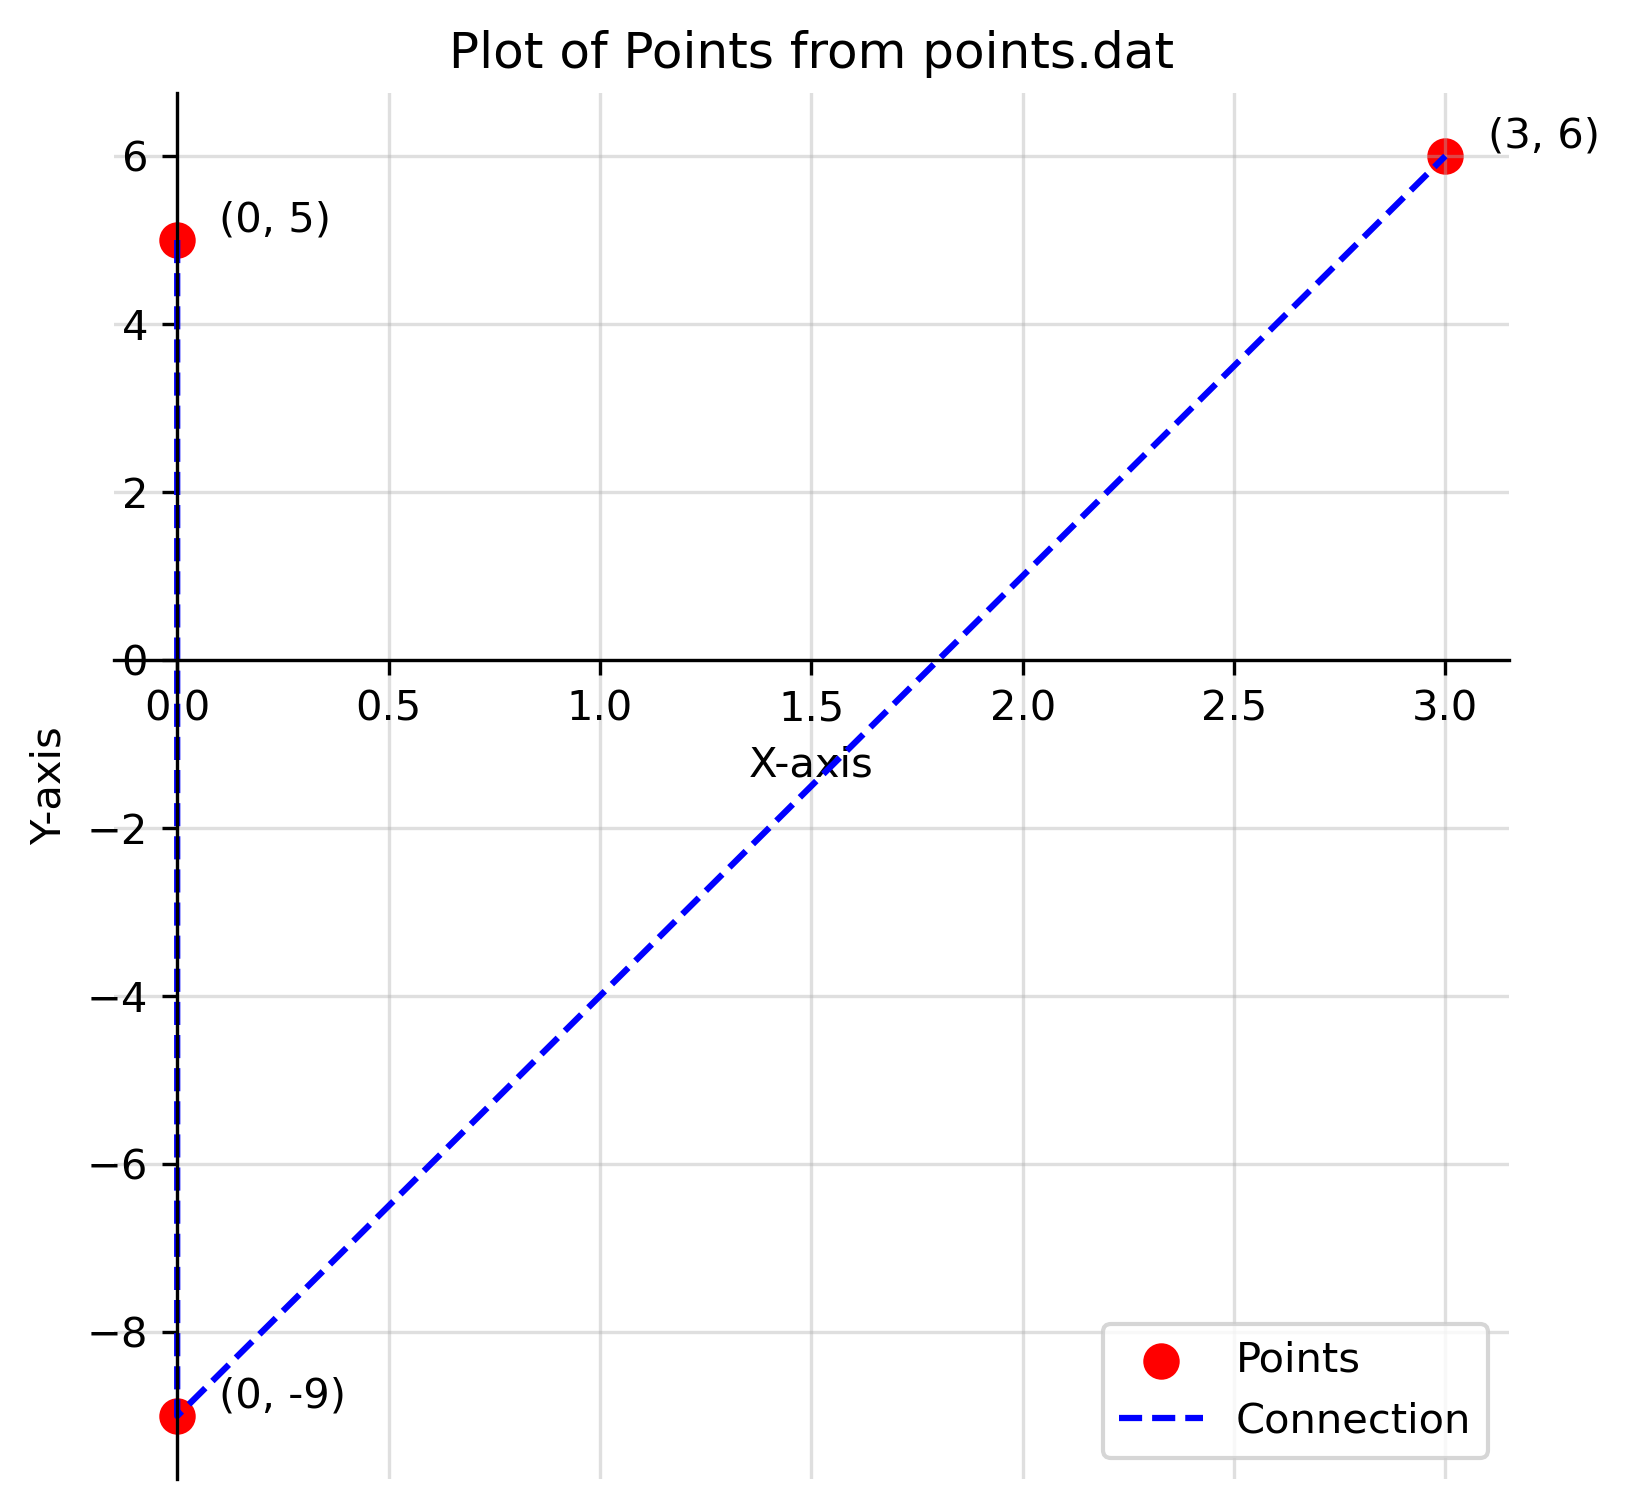
\includegraphics[width=0.5\linewidth]{figs/01.png}
   \caption{A,B,C are not collinear}
   \label{}
\end{figure}
\end{frame}
 % --------- CODE APPENDIX ---------
\section*{Appendix: Code}

% C program
\begin{frame}[fragile]{C Code: points.c}
\begin{lstlisting}[language=C]
#include <stdio.h>

int main() {
  FILE *fp;

  // -------------------
  // Question 1.6.13
  // -------------------


  fp = fopen("points.dat", "w");
  fprintf(fp, "%d,%d,%d\n", 0, 5, 0);  // A
  fprintf(fp, "%d,%d,%d\n", 0, -9, 0);   // B
  fprintf(fp, "%d,%d,%d\n", 3, 6, 0); // C
  fclose(fp);
  return 0;
  }
\end{lstlisting}
\end{frame}

% Python calling C
\begin{frame}[fragile]{Python: call\_c.py}
\begin{lstlisting}[language=Python]
import subprocess

# Compile the C program
subprocess.run(["gcc", "points.c", "-o", "points"])

# Run the compiled C program
result = subprocess.run(["./points"], capture_output=True, text=True)

# Print the output from the C program
print(result.stdout)
\end{lstlisting}
\end{frame}

% Python plotting
\begin{frame}[fragile]{Python: plot.py}
\begin{lstlisting}[language=Python]
import numpy as np
import matplotlib.pyplot as plt

# Load the file, using comma as delimiter
points = np.loadtxt("points.dat", delimiter=",")

# Take only the first two columns (x, y)
x = points[:, 0]
y = points[:, 1]

# --- Plot ---
plt.figure(figsize=(6, 6))
plt.scatter(x, y, color="red", s=60, label="Points")
plt.plot(x, y, linestyle="--", color="blue", label="Connection")

# Annotate each point
for xi, yi in zip(x, y):
    plt.text(xi + 0.1, yi + 0.1, f"({xi:g}, {yi:g})")

# Axes setup
ax = plt.gca()
ax.spines["left"].set_position("zero")
ax.spines["bottom"].set_position("zero")
ax.spines["right"].set_color("none")
ax.spines["top"].set_color("none")

plt.xlabel("X-axis")
plt.ylabel("Y-axis")
plt.title("Plot of Points from points.dat")
plt.grid(True, alpha=0.4)
plt.legend()

# Save the figure
\end{lstlisting}
\end{frame}
% Python plotting
\begin{frame}[fragile]{Python: plot.py }
\begin{lstlisting}[language=Python]
plt.savefig("points_plot.png", dpi=300, bbox_inches="tight")

# Show the figure
plt.show()
\end{lstlisting}
\end{frame}


\end{document}
